%%%%%%%%%%%%%%%%%%%%%%%%%%%%%%%%%%%%%%%%%%%%%%%%%%%%%%%%%%%%%%%%%%%%%%%%%%%%%%%%%
%																				%
%	TRABAJO:	Trabajo Final													%
%				Especialidad en Ingenier�a en Sistemas de Informaci�n			%
%																				%
%		Titulo:																	%
%																				%
%		Autores:	Julian Nonino												%
%																				%
%	Capitulo sobre Procesamiento de Datos en Tiempo Real						%	
%																				%
%	A�o: 2016																	%
%																				%
%%%%%%%%%%%%%%%%%%%%%%%%%%%%%%%%%%%%%%%%%%%%%%%%%%%%%%%%%%%%%%%%%%%%%%%%%%%%%%%%%

\chapter{Procesamiento de Datos en Tiempo Real}
\label{chapter_real_time}

En los �ltimos tiempos, la demanda de procesamiento de flujos continuos de datos
(data streams) se ha incrementado considerablemente. Esto se debe a que ya no es
suficiente con procesar grandes vol�menes de datos. Los datos, adem�s, deben ser
procesados r�pidamente permitiendo a los sistemas reaccionar ante los eventos lo
antes posible. Ejemplos de sistemas que necesitan �ste nivel de procesamiento
son los sistemas de detecci�n de fraude, monitoreo de recursos, comercio,
etc�tera.

\section{Big Data}

	El t�rmino Big Data, muy utilizado en la actualidad, hace referencia a lo que
	se conoce como las tres V, Volumen, Variedad y Velocidad. Con ello, se quiere
	indicar que un sistema Big Data no solo implica trabajar con grandes vol�menes
	de datos, sino que estos datos pueden ser muy variados y se deben procesar
	r�pidamente \cite{Wahner2014}.

	\begin{figure}[H]
		\centering
		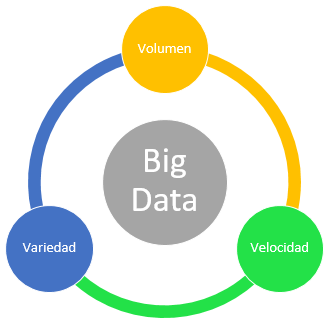
\includegraphics[width=.5\linewidth]{./marco_teorico/img/real_time/big_data_tres_v}
	\end{figure}

\section{Procesamiento de Flujos de Datos (Stream Processing)}
	
	Es un sistema dise�ado para analizar y actuar en tiempo real un flujo continuo
	de datos. En contraste a los modelos de procesamiento de datos tradicionales en
	los cuales los datos son primero almacenados y luego procesados y analizados,
	cuando se procesa un flujo de datos, los datos son procesados y analizados
	mientras entran en el sistema. Esto permite lo que se llama procesar datos en
	movimiento. Esto permite conectar a los procesadores de datos a fuentes de
	datos externas introduciendo a los mismos al flujo de procesamiento.
		
	Una soluci�n de procesamiento de datos en tiempo real debe ser capaz de:
	\begin{itemize}
	    \item Procesar cantidades enormes de datos permitiendo filtrado,
	    agregaci�n, predicci�n, alertas, reglas, etc�tera.
		\item Respuesta en tiempo real a los mensajes/eventos recibdos.
		\item Asegurar rendimiento y escalabilidad cuando el volumen de datos crece en
		tama�o y/o complejidad.
		\item Integraci�n f�cil y r�pida con la infraestructura y fuentes de datos
		existentes.
		\item R�pida implementaci�n y puesta en producci�n de nuevos requisitos de
		procesamiento.
	\end{itemize}
